\documentclass[10pt]{article}
\usepackage{tikz}
\usetikzlibrary{shapes.misc}
\usepackage[margin=0cm]{geometry}
\pagestyle{empty}
\tikzstyle{every node}=[cross out, draw, red]

\begin{document}

\vspace*{\fill}
\begin{center}
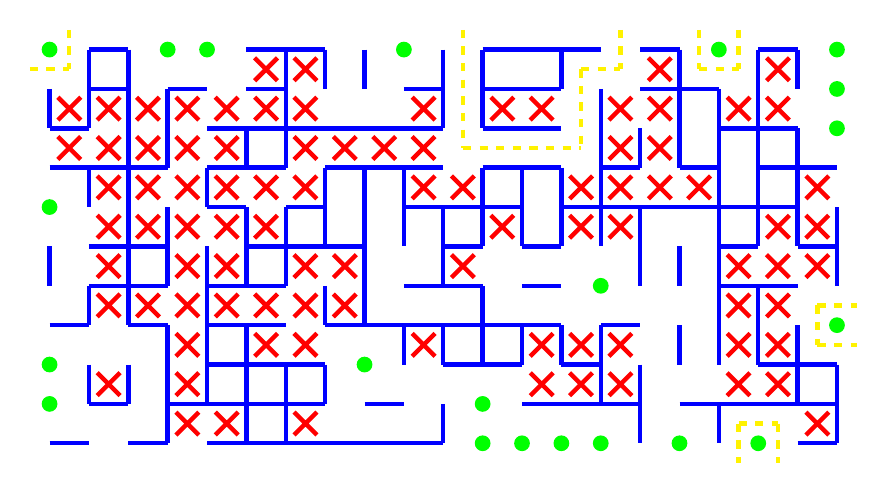
\begin{tikzpicture}[x=0.5cm, y=-0.5cm, ultra thick, blue]
% Walls
    \draw (1,0) -- (2,0);
    \draw (5,0) -- (7,0);
    \draw (11,0) -- (14,0);
    \draw (15,0) -- (16,0);
    \draw (18,0) -- (19,0);
    \draw (1,1) -- (2,1);
    \draw (3,1) -- (4,1);
    \draw (5,1) -- (6,1);
    \draw (9,1) -- (10,1);
    \draw (11,1) -- (13,1);
    \draw (15,1) -- (17,1);
    \draw (0,2) -- (1,2);
    \draw (4,2) -- (10,2);
    \draw (11,2) -- (13,2);
    \draw (17,2) -- (19,2);
    \draw (0,3) -- (3,3);
    \draw (4,3) -- (6,3);
    \draw (7,3) -- (10,3);
    \draw (11,3) -- (13,3);
    \draw (14,3) -- (15,3);
    \draw (16,3) -- (17,3);
    \draw (18,3) -- (20,3);
    \draw (4,4) -- (5,4);
    \draw (6,4) -- (7,4);
    \draw (9,4) -- (12,4);
    \draw (13,4) -- (19,4);
    \draw (1,5) -- (3,5);
    \draw (5,5) -- (8,5);
    \draw (10,5) -- (11,5);
    \draw (12,5) -- (13,5);
    \draw (17,5) -- (18,5);
    \draw (19,5) -- (20,5);
    \draw (1,6) -- (3,6);
    \draw (4,6) -- (6,6);
    \draw (9,6) -- (11,6);
    \draw (12,6) -- (13,6);
    \draw (17,6) -- (19,6);
    \draw (0,7) -- (1,7);
    \draw (2,7) -- (3,7);
    \draw (4,7) -- (6,7);
    \draw (7,7) -- (13,7);
    \draw (14,7) -- (15,7);
    \draw (4,8) -- (7,8);
    \draw (10,8) -- (12,8);
    \draw (13,8) -- (14,8);
    \draw (18,8) -- (20,8);
    \draw (1,9) -- (2,9);
    \draw (3,9) -- (7,9);
    \draw (8,9) -- (9,9);
    \draw (12,9) -- (15,9);
    \draw (16,9) -- (20,9);
    \draw (0,10) -- (1,10);
    \draw (2,10) -- (3,10);
    \draw (4,10) -- (10,10);
    \draw (19,10) -- (20,10);
    \draw (0,1) -- (0,2);
    \draw (0,5) -- (0,6);
    \draw (1,0) -- (1,2);
    \draw (1,3) -- (1,4);
    \draw (1,6) -- (1,7);
    \draw (1,8) -- (1,9);
    \draw (2,0) -- (2,7);
    \draw (2,8) -- (2,9);
    \draw (3,1) -- (3,3);
    \draw (3,4) -- (3,6);
    \draw (3,7) -- (3,10);
    \draw (4,3) -- (4,4);
    \draw (4,5) -- (4,9);
    \draw (5,2) -- (5,3);
    \draw (5,4) -- (5,6);
    \draw (5,7) -- (5,10);
    \draw (6,0) -- (6,3);
    \draw (6,4) -- (6,6);
    \draw (6,8) -- (6,10);
    \draw (7,0) -- (7,1);
    \draw (7,3) -- (7,5);
    \draw (7,6) -- (7,7);
    \draw (7,8) -- (7,9);
    \draw (8,0) -- (8,1);
    \draw (8,3) -- (8,7);
    \draw (9,3) -- (9,5);
    \draw (9,7) -- (9,8);
    \draw (10,0) -- (10,2);
    \draw (10,4) -- (10,6);
    \draw (10,7) -- (10,8);
    \draw (10,9) -- (10,10);
    \draw (11,0) -- (11,2);
    \draw (11,3) -- (11,5);
    \draw (11,6) -- (11,8);
    \draw (12,3) -- (12,5);
    \draw (12,7) -- (12,8);
    \draw (13,0) -- (13,1);
    \draw (13,3) -- (13,5);
    \draw (13,7) -- (13,8);
    \draw (14,1) -- (14,5);
    \draw (14,7) -- (14,9);
    \draw (15,2) -- (15,3);
    \draw (15,4) -- (15,6);
    \draw (15,8) -- (15,10);
    \draw (16,0) -- (16,3);
    \draw (16,5) -- (16,6);
    \draw (16,7) -- (16,8);
    \draw (17,1) -- (17,8);
    \draw (17,9) -- (17,10);
    \draw (18,0) -- (18,5);
    \draw (18,6) -- (18,8);
    \draw (19,0) -- (19,1);
    \draw (19,2) -- (19,5);
    \draw (19,7) -- (19,9);
    \draw (20,4) -- (20,6);
    \draw (20,8) -- (20,10);
% Pillars
    \fill[green] (0,0) circle(0.2);
    \fill[green] (3,0) circle(0.2);
    \fill[green] (4,0) circle(0.2);
    \fill[green] (9,0) circle(0.2);
    \fill[green] (17,0) circle(0.2);
    \fill[green] (20,0) circle(0.2);
    \fill[green] (20,1) circle(0.2);
    \fill[green] (20,2) circle(0.2);
    \fill[green] (0,4) circle(0.2);
    \fill[green] (14,6) circle(0.2);
    \fill[green] (20,7) circle(0.2);
    \fill[green] (0,8) circle(0.2);
    \fill[green] (8,8) circle(0.2);
    \fill[green] (0,9) circle(0.2);
    \fill[green] (11,9) circle(0.2);
    \fill[green] (11,10) circle(0.2);
    \fill[green] (12,10) circle(0.2);
    \fill[green] (13,10) circle(0.2);
    \fill[green] (14,10) circle(0.2);
    \fill[green] (16,10) circle(0.2);
    \fill[green] (18,10) circle(0.2);
% Inner points in accessible cul-de-sacs
    \node at (5.5,0.5) {};
    \node at (6.5,0.5) {};
    \node at (15.5,0.5) {};
    \node at (18.5,0.5) {};
    \node at (0.5,1.5) {};
    \node at (1.5,1.5) {};
    \node at (2.5,1.5) {};
    \node at (3.5,1.5) {};
    \node at (4.5,1.5) {};
    \node at (5.5,1.5) {};
    \node at (6.5,1.5) {};
    \node at (9.5,1.5) {};
    \node at (11.5,1.5) {};
    \node at (12.5,1.5) {};
    \node at (14.5,1.5) {};
    \node at (15.5,1.5) {};
    \node at (17.5,1.5) {};
    \node at (18.5,1.5) {};
    \node at (0.5,2.5) {};
    \node at (1.5,2.5) {};
    \node at (2.5,2.5) {};
    \node at (3.5,2.5) {};
    \node at (4.5,2.5) {};
    \node at (6.5,2.5) {};
    \node at (7.5,2.5) {};
    \node at (8.5,2.5) {};
    \node at (9.5,2.5) {};
    \node at (14.5,2.5) {};
    \node at (15.5,2.5) {};
    \node at (1.5,3.5) {};
    \node at (2.5,3.5) {};
    \node at (3.5,3.5) {};
    \node at (4.5,3.5) {};
    \node at (5.5,3.5) {};
    \node at (6.5,3.5) {};
    \node at (9.5,3.5) {};
    \node at (10.5,3.5) {};
    \node at (13.5,3.5) {};
    \node at (14.5,3.5) {};
    \node at (15.5,3.5) {};
    \node at (16.5,3.5) {};
    \node at (19.5,3.5) {};
    \node at (1.5,4.5) {};
    \node at (2.5,4.5) {};
    \node at (3.5,4.5) {};
    \node at (4.5,4.5) {};
    \node at (5.5,4.5) {};
    \node at (11.5,4.5) {};
    \node at (13.5,4.5) {};
    \node at (14.5,4.5) {};
    \node at (18.5,4.5) {};
    \node at (19.5,4.5) {};
    \node at (1.5,5.5) {};
    \node at (3.5,5.5) {};
    \node at (4.5,5.5) {};
    \node at (6.5,5.5) {};
    \node at (7.5,5.5) {};
    \node at (10.5,5.5) {};
    \node at (17.5,5.5) {};
    \node at (18.5,5.5) {};
    \node at (19.5,5.5) {};
    \node at (1.5,6.5) {};
    \node at (2.5,6.5) {};
    \node at (3.5,6.5) {};
    \node at (4.5,6.5) {};
    \node at (5.5,6.5) {};
    \node at (6.5,6.5) {};
    \node at (7.5,6.5) {};
    \node at (17.5,6.5) {};
    \node at (18.5,6.5) {};
    \node at (3.5,7.5) {};
    \node at (5.5,7.5) {};
    \node at (6.5,7.5) {};
    \node at (9.5,7.5) {};
    \node at (12.5,7.5) {};
    \node at (13.5,7.5) {};
    \node at (14.5,7.5) {};
    \node at (17.5,7.5) {};
    \node at (18.5,7.5) {};
    \node at (1.5,8.5) {};
    \node at (3.5,8.5) {};
    \node at (12.5,8.5) {};
    \node at (13.5,8.5) {};
    \node at (14.5,8.5) {};
    \node at (17.5,8.5) {};
    \node at (18.5,8.5) {};
    \node at (3.5,9.5) {};
    \node at (4.5,9.5) {};
    \node at (6.5,9.5) {};
    \node at (19.5,9.5) {};
% Entry-exit paths without intersections
    \draw[dashed, yellow] (-0.5,0.5) -- (0.5,0.5);
    \draw[dashed, yellow] (13.5,0.5) -- (14.5,0.5);
    \draw[dashed, yellow] (16.5,0.5) -- (17.5,0.5);
    \draw[dashed, yellow] (10.5,2.5) -- (13.5,2.5);
    \draw[dashed, yellow] (19.5,6.5) -- (20.5,6.5);
    \draw[dashed, yellow] (19.5,7.5) -- (20.5,7.5);
    \draw[dashed, yellow] (17.5,9.5) -- (18.5,9.5);
    \draw[dashed, yellow] (0.5,-0.5) -- (0.5,0.5);
    \draw[dashed, yellow] (10.5,-0.5) -- (10.5,2.5);
    \draw[dashed, yellow] (13.5,0.5) -- (13.5,2.5);
    \draw[dashed, yellow] (14.5,-0.5) -- (14.5,0.5);
    \draw[dashed, yellow] (16.5,-0.5) -- (16.5,0.5);
    \draw[dashed, yellow] (17.5,-0.5) -- (17.5,0.5);
    \draw[dashed, yellow] (17.5,9.5) -- (17.5,10.5);
    \draw[dashed, yellow] (18.5,9.5) -- (18.5,10.5);
    \draw[dashed, yellow] (19.5,6.5) -- (19.5,7.5);
\end{tikzpicture}
\end{center}
\vspace*{\fill}

\end{document}
